\section{921 --- Minimum Add to Make Parentheses Valid}
Given a string S of ( and ) parentheses, we add the minimum number of parentheses ( '(' or ')', and in any positions ) so that the resulting parentheses string is valid.
\par
Formally, a parentheses string is valid if and only if:
\begin{itemize}
    \item It is the empty string, or
    \item It can be written as $AB$ ($A$ concatenated with $B$), where $A$ and $B$ are valid strings, or
    \item It can be written as $(A)$, where $A$ is a valid string.
\end{itemize}
Given a parentheses string, return the minimum number of parentheses we must add to make the resulting string valid.
\paragraph{Example 1:}
\begin{flushleft}
Input:
\par
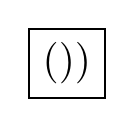
\begin{tikzpicture}[thick,scale=1.5, every node/.style={scale=1.5}]
\node[draw, rectangle, minimum size=3mm] {$())$};
\end{tikzpicture}
\par
Output: 1
\end{flushleft}
\paragraph{Example 2:}
\begin{flushleft}
Input:
\par
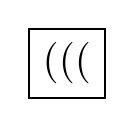
\begin{tikzpicture}[thick,scale=1.5, every node/.style={scale=1.5}]
\node[draw, rectangle, minimum size=3mm] {$((($};
\end{tikzpicture}
\par
Output: 3
\end{flushleft}
\paragraph{Example 3:}
\begin{flushleft}
Input:
\par
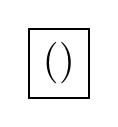
\begin{tikzpicture}[thick,scale=1.5, every node/.style={scale=1.5}]
\node[draw, rectangle, minimum size=3mm] {$()$};
\end{tikzpicture}
\par
Output: 0
\end{flushleft}
\paragraph{Example 4:}
\begin{flushleft}
Input:
\par
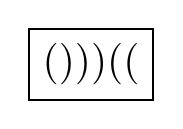
\begin{tikzpicture}[thick,scale=1.5, every node/.style={scale=1.5}]
\node[draw, rectangle, minimum size=6mm] {$()))(($};
\end{tikzpicture}
\par
Output: 4
\end{flushleft}
\paragraph{Note:}
\begin{flushleft}
$|S| \leq 1000$
\par
S only consists of \textbf{(} and \textbf{)} characters.
\end{flushleft}
\subsection{Linear Scan}
\begin{CJK*}{UTF8}{gbsn}
比较简单的题,用两个计数器$\alpha$和$\beta$分别记录遇到的左括号和右括号的个数,当遇到左括号时,$\alpha \gets \alpha+1$, 当遇到右括号时,先看当前的$\alpha$是否为0,如果不为0,$\alpha \gets \alpha-1$,表示我们可以用当前遇到的右括号去和之前的左括号形成valid string。如果为0, 则$\beta \gets \beta -1 $。最后,返回 $\alpha + \beta$
\end{CJK*}
\subsubsection{Algorithm}
The inputs of the following procedure are:
\begin{itemize}
    \item $S$ --- The input string
    \item $N$ --- The length of $S$
\end{itemize}
\setcounter{algorithm}{0}
\begin{algorithm}[H]
\caption{Linear Scan Based Solution}
\begin{algorithmic}[1]
\Procedure{MinAddToMakeValid}{$S$, $N$}
\State $\alpha:=0$ \Comment The count of left parenthesis
\State $\beta :=0$ \Comment The count of right parenthesis
\For{$c \in S$} \Comment Iterate over characters in $S$
\If{$c = ($} \Comment Found left parenthesis \label{921if0}
\State $\alpha \gets \alpha + 1$
\Else \Comment Found right parenthesis
\If{$\alpha > 0$} \Comment We have pending left parenthesis \label{921if1}
\State $\alpha \gets \alpha - 1$
\Else
\State $\beta \gets \beta + 1$
\EndIf \Comment End[\ref{921if1}]
\EndIf \Comment End[\ref{921if0}]
\EndFor
\State \Return $\alpha + \beta$
\EndProcedure
\end{algorithmic}
\end{algorithm}

\section{922 --- Sort Array By Parity II}
Given an array $A$ of non-negative integers, half of the integers in $A$ are odd, and half of the integers are even.
\par
Sort the array so that whenever $A[i]$ is odd, $i$ is odd; and whenever $A[i]$ is even, $i$ is even.
\par
You may return any answer array that satisfies this condition.
\paragraph{Example 1:}
 \begin{flushleft}
\textbf{Input}: $[4,2,5,7]$
\par
\textbf{Output}: $[4,5,2,7]$
\par
\textbf{Explanation}: $[4,7,2,5]$, $[2,5,4,7]$, $[2,7,4,5]$ would also have been accepted. 
 \end{flushleft}
\paragraph{Note:}
\begin{flushleft}
$2 \leq |A| \leq 20000$
\par
$|A| \bmod 2 \equiv 0$
\par
$0\leq A[i] \leq 1000$
\end{flushleft}
\subsection{In Place Swap}
Suppose we have $\alpha$ and $\beta$ to track even and odd indexes separately. When we meet a number at current $\alpha$ is odd, we just search from current $\beta$ to find the first \textbf{even} number in a {\color{red}odd} index, and then swap them. Likely, when a number at current $\beta$ is even, search from current $\alpha$ to find the first \textbf{odd} number in an {\color{red}even} index, and then swap. 
\subsubsection{Algorithm}
The inputs of the following procedure are:
\begin{itemize}
    \item $A$ --- The input array
    \item $N$ --- The length of $A$
\end{itemize}
\setcounter{algorithm}{0}
\begin{algorithm}[H]
\caption{In-place Swap Based Solution}
\begin{algorithmic}[1]
\Procedure{SortArrayByParityII}{$A$, $N$}
\State $\alpha := 0$ \Comment Even index tracker
\State $\beta := 1$ \Comment Odd index tracker
\While{$\alpha < N$ \textbf{and} $\beta < N$}
\If{$A[\alpha] \bmod 2 = 1$} \Comment Found a odd number in a even index \label{922if1}
\While{$\beta < N$ \textbf{and} $A[\beta] \bmod 2 = 1$}
\State $\beta \gets \beta + 2$ \Comment Continue to next odd index
\EndWhile
\If{$\beta < N$} \Comment Found a even number in a odd index
\State $A[\alpha] \Longleftrightarrow A[\beta]$ \Comment Exchange $A[\alpha]$ with $A[\beta]$
\EndIf
\EndIf \Comment End [\ref{922if1}]
\State $\alpha \gets \alpha + 2 $ \Comment Continue to next even index
\If{$A[\beta] \bmod 2 = 0$} \Comment Found a even number in a odd index \label{922if2}
\While{$\alpha < N$ \textbf{and} $A[\alpha] \bmod 2 = 0$}
\State $\alpha \gets \alpha + 2$ \Comment Continue to next odd index
\EndWhile
\If{$\alpha < N$} \Comment Found a odd number in a even index
\State $A[\beta] \Longleftrightarrow A[\alpha]$ \Comment Exchange $A[\beta]$ with $A[\alpha]$
\EndIf
\EndIf \Comment End [\ref{922if2}]
\State $\beta \gets \beta + 2 $ \Comment Continue to next odd index
\EndWhile
\State \Return $A$ \Comment Return the modified input array $A$
\EndProcedure
\end{algorithmic}
\end{algorithm}

\section{923 --- 3Sum With Multiplicity}
Given an integer array $A$, and an integer target $T$, return the number of tuples $i, j, k$  such that $i < j < k$ and $A[i] + A[j] + A[k] = T$.
\par
As the answer can be very large, return it modulo $10^9 + 7$.
\paragraph{Example 1:}
\begin{flushleft}
\textbf{Input}: $A = [1,1,2,2,3,3,4,4,5,5]$, $T = 8$
\par
\textbf{Output}: 20
\par
\textbf{Explanation}:
\par
Enumerating by the values $(A[i], A[j], A[k])$:
\par
$(1, 2, 5)$ occurs 8 times;
$(1, 3, 4)$ occurs 8 times;
$(2, 2, 4)$ occurs 2 times;
$(2, 3, 3)$ occurs 2 times.
\end{flushleft}
\paragraph{Example 2:}
\begin{flushleft}
\textbf{Input}: $A = [1,1,2,2,2,2]$, $T = 5$
\par
\textbf{Output}: 12
\par
\textbf{Explanation}: 
\par
$A[i] = 1$,$A[j] = A[k] = 2$ occurs 12 times:
\par
We choose one 1 from $[1,1]$ in 2 ways,
\par
and two 2s from $[2,2,2,2]$ in 6 ways.
\end{flushleft}
\paragraph{Note:}
\begin{flushleft}
$3 \leq |A| \leq 3000$
\par
$0 \leq A[i] \leq 100$
\par
$0 \leq T \leq 300$
\end{flushleft}
\subsection{Combinatorics}
Suppose we have $n_1$ $\alpha$, $n_2$ $\beta$ and $n_3$ $\gamma$. Then the total number of counts $\Sigma$ for selecting three numbers with one is $\alpha$, another is $\beta$ and the other is $\gamma$ will be
\[
\Sigma = \binom{n_1}{1} \times \binom{n_2}{1} \times \binom{n_3}{1} = n_1 \times n_2 \times n_3
\]
In this problem, $A[i]$, $A[j]$ and $A[k]$ are different when $i\neq j $ and $j\neq k$. In addition, the problem requires the result be the modular of $10^9+7$. Hence, we need to apply modular to every place where changes the count.
\subsubsection{Algorithm}
The input paramter is the array $A$, its number of elements $N$ and the target $T$
\setcounter{algorithm}{0}
\begin{algorithm}[H]
\caption{Combinatorics Based Solution}
\begin{algorithmic}[1]
\Procedure{ThreeSumMulti}{$A$, $N$, $T$}
\State Sort $A$ so that $A[0]\leq A[1] \leq \ldots \leq A[N-1]$
\State $\theta := 10^9 + 7$
\If{$A[0] = A[N-1]$} \Comment All the numbers are the same
\State \Return $\left[N \bmod \theta \times (N-1)\bmod \theta \times (N-2) \bmod \theta / 6\right] \bmod \theta$ \Comment It is $\binom{N}{3}$
\EndIf
\State $\Sigma:=0$ \Comment The total counts
\For{$i:=0$ \textbf{to} $N-2$}
\State $\beta := T - A[i]$ \Comment Find if $A[l] + A[r] = \beta = T - A[0]$
\State $l:=i+1$
\State $r:=N-1$
\While{$l < r$} \Comment Search candidates in $A[i+1 \ldots N-1]$
\If{$A[l]+A[r] = \beta$} \label{923if1}
\If{$A[l] = A[r]$} \Comment $A[l\ldots r]$ are all same \label{923if0}
\State $\sigma := r-l+1$ \Comment Count of numbers in $A[l\ldots r]$
\State $\Sigma \gets \left[\Sigma + \sigma \bmod \theta \times (\sigma -1) \bmod \theta / 2\right] \bmod \theta$ \Comment $\Sigma \gets \Sigma + \binom{\sigma}{2}$
\State \texttt{break} \Comment Break the loop
\EndIf \Comment End [\ref{923if0}]
\State $(n_1, n_2) := \Gamma(A, l, r)$ \Comment Get count of numbers equal to $A[l]$ and $A[r]$ separately [\ref{923HelperFunc}]
\State $\Sigma \gets \left[\Sigma + n_1 \bmod \theta \times n_2 \bmod \theta\right] \bmod \theta$ \Comment $\Sigma \gets \Sigma + \binom{n_1}{1} \times \binom{n_2}{1}$
\State $l \gets l+1$
\State $r \gets r-1$
\ElsIf{$A[l]+A[r] < \beta$}
\State $l \gets l+1$ \Comment Increase left hand
\Else
\State $r \gets r-1$ \Comment Decrease right hand
\EndIf \Comment End [\ref{923if1}]
\EndWhile
\EndFor
\EndProcedure
\end{algorithmic}
\end{algorithm}
The following is a helper function $\Gamma$ which returns the counts of numbers $n_1$ and $n_2$, where $n_1$ is the count of numbers $A[i] = A[l]$ where $i \in [l, r]$ and $n_2$ the count $A[j] = A[r]$ where $j \in [l, r]$
\begin{algorithm}[H]
\caption{Get Count Of Duplicate Numbers}
\label{923HelperFunc}
\begin{algorithmic}[1]
\Function{$\Gamma$}{$A$, $l$, $r$}
\State $\alpha := l$
\While{$l < r$ \textbf{and} $A[l+1] = A[l]$}
\State $l\gets l+1$ \Comment Increment $l$
\EndWhile
\State $n_1:= l - \alpha + 1$ \Comment Current $l$ is the rightmost element that is equal to $A[\alpha]$
\State $\beta := r$
\While{$l < r$ \textbf{and} $A[r-1] = A[r]$}
\State $r\gets r-1$ \Comment Decrement $r$
\EndWhile
\State $n_2:= \beta -r +1$ \Comment Current $r$ is the leftmost element that is equal to $A[\beta]$
\State \Return $(n_1, n_2)$
\EndFunction
\end{algorithmic}
\end{algorithm}

\section{924 --- Minimize Malware Spread} \label{lc924}
In a network of nodes, each node $i$ is directly connected to another node $j$ if and only if $G[i][j] = 1$.
\par
Some nodes initial are initially infected by malware.  Whenever two nodes are directly connected and at least one of those two nodes is infected by malware, both nodes will be infected by malware.  This spread of malware will continue until no more nodes can be infected in this manner.
\par
Suppose $M(I)$ is the final number of nodes infected with malware in the entire network, after the spread of malware stops.
\par
We will remove one node from the initial list $I$.  Return the node that if removed, would minimize $M(I)$.  If multiple nodes could be removed to minimize $M(I)$, return such a node with the smallest index.
\par
Note that if a node was removed from the initial list of infected nodes, it may still be infected later as a result of the malware spread.
\paragraph{Example 1:}
\begin{flushleft}
\textbf{Input}: $G = [[1,1,0],[1,1,0],[0,0,1]]$, $I = [0,1]$
\par
\textbf{Output}: 0
\end{flushleft}
\paragraph{Example 2:}
\begin{flushleft}
\textbf{Input}: $G = [[1,0,0],[0,1,0],[0,0,1]]$, $I = [0,2]$
\par
\textbf{Output}: 0
\end{flushleft}
\paragraph{Example 3:}
\begin{flushleft}
\textbf{Input}: $G = [[1,1,1],[1,1,1],[1,1,1]]$, $I = [1,2]$
\textbf{Output}: 1
 \end{flushleft}
\paragraph{Note:}
\begin{flushleft}
$1 < |G| = |G[0]| \leq 300$
\par
$0 \leq G[i][j] \leq 1$
\par
$1\leq |I| < |G|$
\par
$0 \leq I[i] < |G|$
\end{flushleft}

\subsection{Depth First Search}
This is actually ask for what is the smallest node which has most nodes in its connected components. We can use either depth first search or union.
\par
In DFS approach, an auxiliary array $\alpha$ is provided to mark a node $i$'s color. The node $i$'s color is the connected node id $\gamma$ in the initial list.
\subsubsection{Algorithm}
The input includes the graph $M$, the number of nodes $N$ and the initial list $I$
\setcounter{algorithm}{0}
\begin{algorithm}[H]
\caption{DFS Based Solution}
\begin{algorithmic}[1]
\Procedure{MinMalwareSpread}{$M$, $N$, $I$}
\State $\alpha$ as $\alpha[0] = \ldots = \alpha[N-1] := -1$ 
\State $\Sigma := 0$ \Comment The maximum number of connected nodes so far.
\State $\beta := -1$ \Comment The id of the node which has $\Sigma$ in its connected component
\State $\mu:= -1$ \Comment The smallest id of the node in the connected component that has $\Sigma$
\For{$i:= n \in I $} \Comment Iterate over all nodes in $I$ \label{924for1}
\If{$\alpha[n] = -1$} \Comment This node has not been visited \label{924if3}
\State $\sigma := 0$ \Comment The number of nodes in the current connected component
\State $\mathtt{DFS}(M, \alpha, N, i, i, \sigma)$ \Comment Call function [\ref{924DFS}]
\If{$\sigma > \Sigma$} \label{924if2}
\State $\beta \gets i$ \Comment Update to $i$.
\State $\mu \gets i$ \Comment Update to $i$  since it is the first one in its connected component.
\State $\Sigma \gets \sigma$
\ElsIf{$\sigma = \Sigma$}
\If{$\beta > i$} \Comment $i$ is smaller with same number of nodes as $\Sigma$ \label{924if1}
\State $\beta \gets i$
\State $\mu \gets i$
\EndIf \Comment End [\ref{924if1}]
\EndIf \Comment End [\ref{924if2}]
\Else
\If{$\beta = \alpha[i]$ \textbf{and} $i < \mu$} \Comment If $i$ is in the connected component with $\Sigma$
\State $\mu \gets i$ \Comment $i$ is less than the smallest id in this connected component
\EndIf
\EndIf \Comment End [\ref{924if3}]
\EndFor \Comment End [\ref{924for1}]
\State \Return $\mu$
\EndProcedure
\end{algorithmic}
\end{algorithm}

The depth first find function \texttt{DFS} has the following inputs
\begin{itemize}
    \item $M$ --- The input graphic
    \item $\alpha$ --- The auxiliary array to mark the node's color
    \item $N$ --- The number of nodes in the graph
    \item $\lambda$ --- The current starting node
    \item $\gamma$ --- The color id of the connected component
    \item $\sigma$ --- The number of connected nodes
\end{itemize}
\begin{algorithm}[H]
\caption{Find Connected Component By DFS}
\label{924DFS}
\begin{algorithmic}[1]
\Function{DFS}{$M$, $\alpha$, $N$, $\lambda$, $\gamma$, $\Sigma$}
\State $\alpha[\lambda] \gets \gamma$ \Comment Color current node $\lambda$ as the color $\gamma$
\State $\Sigma \gets \Sigma + 1$ \Comment Increment the connected nodes
\For{$i:=0$ \textbf{to} $N-1$}
\If{$M[\lambda][i] = 1$ \textbf{and} $\alpha[i] = -1$ } \Comment If $\lambda$ and $i$ is connected and $i$ is not visited
\State $\mathtt{DFS}(M, \alpha, N, i, \gamma, \sigma)$ \Comment Recursive on next node
\EndIf
\EndFor
\EndFunction
\end{algorithmic}
\end{algorithm}

\section{927 --- Three Equal Parts}
Given an array $A$ of 0s and 1s, divide the array into 3 non-empty parts such that all of these parts represent the same binary value.
\par
If it is possible, return any $[i, j]$ with $i+1 < j$, such that:
\begin{itemize}
    \item $A[0], A[1], \ldots, A[i]$ is the first part;
    \item $A[i+1], A[i+2], \ldots, A[j-1]$ is the second part, and
    \item $A[j], A[j+1], ..., A[|A| - 1]$ is the third part.
    \item All three parts have equal binary value.
\end{itemize}
\par
If it is not possible, return [-1, -1].
\par
Note that the entire part is used when considering what binary value it represents.  For example, $[1,1,0]$ represents 6 in decimal, not 3.  Also, leading zeros are allowed, so [0,1,1] and [1,1] represent the same value.
\paragraph{Example 1:}
\begin{flushleft}
\textbf{Input}: $[1,0,1,0,1]$
\\
\textbf{Output}: $[0,3]$
\end{flushleft}
\paragraph{Example 2:}
\begin{flushleft}
\textbf{Input}: $[1,1,0,1,1]$
\\
\textbf{Output}: $[-1,-1]$
\end{flushleft}
\paragraph{Note:}
\begin{flushleft}
$3 \leq |A| \leq 30000$
\\
$A[i] == 0$ or $A[i] == 1$
\end{flushleft}
\subsection{Equal Ones}
\begin{CJK*}{UTF8}{gbsn}
很显然这3个区间若要有相同的二进制表达式,1的个数必须相等,这是必要条件。首先找到所有的1的个数,然后看能否被3整除,如果不能就直接退出。设每段区间的1的个数为$\sigma$。然后扫描数组,找到如下的index
\begin{itemize}
\item $\alpha_1$ --- 第一个1出现的位置
\item $\beta_1$ --- 第$\sigma$个1出现的位置
\item $\alpha_2$ --- 第$\sigma+1$出现的位置
\item $\beta_2$ --- 第$2\times\sigma$个1出现的位置
\item $\alpha_3$ --- 第$2\times\sigma+1$出现的位置
\item $\beta_3$ --- 第$3\times\sigma$个1出现的位置
\end{itemize}
这样$A$就分割成了如下区间
\begin{figure}[H]
\begin{tikzpicture}[minimum width = 0.5cm, minimum height = 1cm, text=violet]
\node(0){};
\node(1) at (0.5,0) {$[0\ldots0]$};
\node(2) [right=0.2cm of 1] {$[A[\alpha_1]\ldots A[\beta_1]]$};
\node(3) [right=0.2cm of 2] {$[0\ldots0]$};
\node(4) [right=0.2cm of 3] {$[A[\alpha_2]\ldots A[\beta_2]]$};
\node(5) [right=0.2cm of 4] {$[0\ldots0]$};
\node(6) [right=0.2cm of 5] {$[A[\alpha_3]\ldots A[\beta_3]]$};
\node(7) [right=0.2cm of 6] {$[0\ldots0]$};
\end{tikzpicture}
\end{figure}
\par
接着进行分段数组比较,因为leading zeros也是可以包含在内的,所以比较数组是否是相同的binary表达式只能从第一个1开始比较,因此也就是比较
\begin{align*}
&(A[\alpha_1]\ldots A[\beta_1]0\ldots0)\\
&(A[\alpha_2]\ldots A[\beta_2]0\ldots0)\\
&(A[\alpha_3]\ldots A[\beta_3]0\ldots0)
\end{align*}

而$(A[\alpha_3]\ldots A[\beta_3]0\ldots0)$是一直到$A$的最后一个element的,所以每段的后面需要比较的0的个数就由最后一段的0的个数来确定,而这个0的个数即为$\delta:=n-1-\beta_3$。也就是说我们其实比较的binary分段数组为
\begin{align*}
&(A[\alpha_1]\ldots A[\beta_1]\underbrace{0\ldots0}_{\delta})\\
&(A[\alpha_2]\ldots A[\beta_2]\underbrace{0\ldots0}_{\delta})\\
&(A[\alpha_3]\ldots A[\beta_3]\underbrace{0\ldots0}_{\delta})
\end{align*}
因此如果全0区间$[\beta_1+1, \alpha_2-1]$和$[\beta_2+1, \alpha_3-1]$中任何一个0的个数小于$\delta$都是不能够形成相同的binary表达式的,因为长度都不够。
\par
如果没有出现这种情况,然后看三个区间$[\alpha_1\ldots\beta_1], [\alpha_2\ldots\beta_2], [\alpha_3\ldots\beta_3]$长度是否相等,如果不相等肯定是不相同的binary表达式。
\par
最后再逐个元素比较这三个分段数组是否都是相同的,如果是那么根据题目中分界点$i,j$的定义最后得到的两个分界点index分别是$i=\beta_1 + \delta$和$j=\beta_2+\delta+1$。
\par
有一个边界case,是$A$中所有element都是0,这时候返回0和$n-1$即可,$n$为$A$的长度。
\end{CJK*}
\subsubsection{Algorithm}
The inputs of the following procedure include:
\begin{itemize}
\item $A$ --- The input array
\item $n$ --- The length of $A$
\end{itemize}
\setcounter{algorithm}{0}
\begin{algorithm}[H]
\caption{Count Equal Ones Approach}
\begin{algorithmic}[1]
\Procedure{ThreeEqualParts}{$A, n$}
\State $C:=0$ \Comment The count of 1s in $A$
\For{$i:0$ \textbf{to} $n-1$}
\State $C\gets C+A[i]$ \Comment $A$ is $0/1$ array
\EndFor
\If{$C\bmod 3 \neq 0$} \Comment The counts of 1 is not multiple of 3
\State \Return $[-1,-1]$
\EndIf
\If{$C=0$} \Comment $A$ are all 0s
\State \Return $[0,n-1]$
\EndIf
\State $\sigma := C / 3$ \Comment The number of 1s in each segment
\State $\alpha_1:=-1, \beta_1:=-1, \alpha_2:=-1, \beta_2:=-1,\alpha_3:=-1, \beta_3:=-1$
\State $C\gets 0$
\For{$i:=0$ \textbf{to} $n-1$} \label{927for1}
\If{$A[i] = 1$} \label{927if1}
\State $C\gets C+1$
\If{$C = 1$}
\State $\alpha_1 \gets i$ \Comment The 1st 1
\EndIf
\If{$C = \sigma$}
\State $\beta_1 \gets i$ \Comment The $\sigma$-st 1
\EndIf
\If{$C = \sigma+1$}
\State $\alpha_2 \gets i$ \Comment The $\sigma+1$-st 1
\EndIf
\If{$C = 2\times \sigma$}
\State $\beta_2 \gets i$ \Comment The $2\times\sigma$-st 1
\EndIf
\algstore{927algo}
\end{algorithmic}
\end{algorithm}

\begin{algorithm}[H]
\begin{algorithmic}[1]
\algrestore{927algo}
\If{$C = 2\times\sigma + 1$}
\State $\alpha_3 \gets i$ \Comment The $2\times\sigma+1$-st 1
\EndIf
\If{$C = 3\times\sigma$}
\State $\beta_3 \gets i$ \Comment The $3\times\sigma$-st 1
\EndIf
\EndIf \Comment End[\ref{927if1}]
\EndFor \Comment End[\ref{927for1}]
\State $\delta := n-1-\beta3$ \Comment The suffix zeros to be compared
\If{$\alpha_2 - 1 - \beta_1 < \delta$ \textbf{or} $\alpha_3 - 1 - \beta_2 < \delta$} \Comment Do not have enough zeros to compare
\State \Return $[-1,-1]$
\EndIf
\If{$\beta_1 - \alpha_1 \neq \beta_2 - \alpha_2$ \textbf{or} $\beta_2 - \alpha_2 \neq \beta_3 - \alpha_3$}
\State \Return $[-1,-1]$ \Comment The length of each segment is not equal
\EndIf
\State $l:=\beta_1 - \alpha_1$
\For{$i:=0$ \textbf{to} $l$} \Comment Compare element each by each
\If{$A[i+\alpha_1] \neq A[i+\alpha_2]$ \textbf{or} $A[i+\alpha_2] \neq A[i+\alpha_3]$ }
\State \Return $[-1,-1]$ \Comment Found different element
\EndIf
\EndFor
\State \Return $[\beta_1+\delta, \beta_2+\delta+1]$ \Comment The separate index
\EndProcedure
\end{algorithmic}
\end{algorithm}

\section{928 --- Minimize Malware Spread II}
This problem is the same as [\ref{lc924}], with the differences bolded.
\par
In a network of nodes, each node $i$ is directly connected to another node $j$ if and only if $G[i][j] = 1$.
\par
Some nodes initial $I$ are initially infected by malware.  Whenever two nodes are directly connected and at least one of those two nodes is infected by malware, both nodes will be infected by malware.  This spread of malware will continue until no more nodes can be infected in this manner.
\par
Suppose $M(I)$ is the final number of nodes infected with malware in the entire network, after the spread of malware stops.
\par
We will remove one node from the initial list, \textbf{completely removing it and any connections from this node to any other node}.  Return the node that if removed, would minimize $M(I)$.  If multiple nodes could be removed to minimize $M(I)$, return such a node with the smallest index.
\paragraph{Example 1:}
\begin{flushleft}
\textbf{Input}:
\\
$G = [[1,1,0],[1,1,0],[0,0,1]], I = [0,1]$
\\
\textbf{Output}: 0
\end{flushleft}
\paragraph{Example 2:}
\begin{flushleft}
\textbf{Input}:
\\
$G = [[1,1,0],[1,1,1],[0,1,1]], I = [0,1]$
\\
\textbf{Output}: 1
\end{flushleft}
\paragraph{Example 3:}
\begin{flushleft}
\textbf{Input}:
\\
$G = graph = [[1,1,0,0],[1,1,1,0],[0,1,1,1],[0,0,1,1]], I = [0,1]$
\\
\textbf{Output}: 1
\end{flushleft}
\paragraph{Note:}
\begin{flushleft}
$1 < |G| = |G[0]| \leq 300$
\\
$0 \leq G[i][j] = G[j][i] \leq 1$
\\
$G[i][i] = 1$
\\
$1 \leq  |I| < |G|$
\\
$0 \leq I[i] <|G|$
\end{flushleft}
\subsection{Depth First Search}
\begin{CJK*}{UTF8}{gbsn}
这道题目和[\ref{lc924}]的不同之处在于,[\ref{lc924}]中的remove某个node其实是把这个node当成没有被感染,仍旧在graph中,在这里需要把node和所有以这个node为一端的edge从$G$中移除,这样就会造成该node所在的\texttt{connected component}发生断裂。
\par
所以,这里采用的方法是,对于$I$中的某个node $n$, 在G中把所有与$n$相连的node $i$ 断开,即如果$G[n][i]=1 \forall (0\leq i\leq N, i\neq n)$,set $G[n][i]=0$。然后进行深度优先搜索,找出在移除$n$的情况下,测试$I$中剩下的每一个node$\alpha$所形成的\texttt{connected component}的大小。然后能够生成最小\texttt{connected component}的$\alpha$就是最优解的candidate.
\par
测试完成后,需要把graph重置回初始状态,然后到下一个$I$中的node继续进行上述的算法流程。
\par
以下图为例,其中$I =(0,1,2)$,以蓝色标记
\begin{figure}[H]
\begin{tikzpicture}
[initial/.style = {minimum size=3mm, draw=blue!75, fill=blue!20, circle},
other/.style = {minimum size=3mm, draw=black!75, fill=black!20, circle}]
\node {};
\node[initial](1) at (2,0) {1};
\node[initial](0) [above = 5mm of 1, xshift=-8mm] {0};
\node[other](7) [below = 5mm of 1, xshift=-8mm] {7};
\node[initial](2) [right = 5mm of 1] {2};
\node[other](3) [right = 5mm of 2] {3};
\node[other](4) [right = 5mm of 3] {4};
\node[other](5) [above = 5mm of 4, xshift = 8mm] {5};
\node[other](6) [below = 5mm of 4, xshift = 8mm] {6};
\draw[-] (0) -- (1);
\draw[-] (1) -- (7);
\draw[-] (1) -- (2);
\draw[-] (2) -- (3);
\draw[-] (3) -- (4);
\draw[-] (4) -- (5);
\draw[-] (4) -- (6);
\end{tikzpicture}
\end{figure}
\par
首先删除node 0,得到下图,红色为被感染的nodes。
\begin{figure}[H]
\begin{tikzpicture}
[initial/.style = {minimum size=3mm, draw=blue!75, fill=blue!20, circle},
other/.style = {minimum size=3mm, draw=black!75, fill=black!20, circle},
malware/.style = {minimum size=3mm, draw=red!75, fill=red!20, circle}]
\node {};
\node[malware](1) at (2,0) {1};
\node(0) [above = 5mm of 1, xshift=-8mm, minimum size=3mm, fill=violet!30, circle] {0};
\node[malware](7) [below = 5mm of 1, xshift=-8mm] {7};
\node[malware](2) [right = 5mm of 1] {2};
\node[malware](3) [right = 5mm of 2] {3};
\node[malware](4) [right = 5mm of 3] {4};
\node[malware](5) [above = 5mm of 4, xshift = 8mm] {5};
\node[malware](6) [below = 5mm of 4, xshift = 8mm] {6};
\draw[-] (1) -- (7);
\draw[-] (1) -- (2);
\draw[-] (2) -- (3);
\draw[-] (3) -- (4);
\draw[-] (4) -- (5);
\draw[-] (4) -- (6);
\end{tikzpicture}
\end{figure}
\par
可以看到这时候感染的nodes数为7。
\par
然后看删除node 1之后会是什么情况,如下图所示
\begin{figure}[H]
\begin{tikzpicture}
[initial/.style = {minimum size=3mm, draw=blue!75, fill=blue!20, circle},
other/.style = {minimum size=3mm, draw=black!75, fill=black!20, circle},
malware/.style = {minimum size=3mm, draw=red!75, fill=red!20, circle}]
\node {};
\node(1) at (2,0) [above = 5mm of 1, xshift=-8mm, minimum size=3mm, fill=violet!30, circle] {1};
\node[malware](0) [above = 5mm of 1, xshift=-8mm]  {0};
\node[other](7) [below = 5mm of 1, xshift=-8mm] {7};
\node[malware](2) [right = 5mm of 1] {2};
\node[malware](3) [right = 5mm of 2] {3};
\node[malware](4) [right = 5mm of 3] {4};
\node[malware](5) [above = 5mm of 4, xshift = 8mm] {5};
\node[malware](6) [below = 5mm of 4, xshift = 8mm] {6};
\draw[-] (2) -- (3);
\draw[-] (3) -- (4);
\draw[-] (4) -- (5);
\draw[-] (4) -- (6);
\end{tikzpicture}
\end{figure}
\par
图中可见,node 1删除后,node 0仍然是被感染的,因为它是处于$I$中的node,而node 7没有被感染。其余节点因为和node 2处于同一个连通区域,所以都被感染。这时候感染的node数为6。因为删除1后感染的node数比删除0后感染的node数少了,因此当前的最佳删除节点是1。
\par
最后看删除节点2的情况,如下图
\begin{figure}[H]
\begin{tikzpicture}
[initial/.style = {minimum size=3mm, draw=blue!75, fill=blue!20, circle},
other/.style = {minimum size=3mm, draw=black!75, fill=black!20, circle},
malware/.style = {minimum size=3mm, draw=red!75, fill=red!20, circle}]
\node {};
\node[malware](1) at (2,0) {1};
\node[malware](0) [above = 5mm of 1, xshift=-8mm] {0};
\node[malware](7) [below = 5mm of 1, xshift=-8mm] {7};
\node(2) [right = 5mm of 1, minimum size=3mm, fill=violet!30, circle] {2};
\node[other](3) [right = 5mm of 2] {3};
\node[other](4) [right = 5mm of 3] {4};
\node[other](5) [above = 5mm of 4, xshift = 8mm] {5};
\node[other](6) [below = 5mm of 4, xshift = 8mm] {6};
\draw[-] (0) -- (1);
\draw[-] (1) -- (7);
\draw[-] (3) -- (4);
\draw[-] (4) -- (5);
\draw[-] (4) -- (6);
\end{tikzpicture}
\end{figure}
\par
图中可以看出,感染的节点只有0,1和7。因此这时候感染的node数为3,因此最佳的删除节点是2。
\end{CJK*}
\subsubsection{Algorithm}
The inputs of the following procedure includes:
\begin{itemize}
    \item $G$ --- The graph matrix
    \item $N$ --- The number of nodes in $G$
    \item $I$ --- The initial node list
\end{itemize}
\setcounter{algorithm}{0}
\begin{algorithm}[H]
\caption{DFS Based Solution}
\begin{algorithmic}[1]
\Procedure{MinMalwareSpread}{$G$, $N$, $I$}
\State $\alpha := \emptyset$ \Comment The temporary array to store nodes.
\State $\Sigma := N$ \Comment The minimum infected nodes so far. Set to maximum value $N$ at first
\State $\beta := -1$ \Comment The node which produce $\Sigma$ nodes by deleteing it
\For{$ n \in I $} \Comment Iterate over each node $n$ in $I$ \label{928for1}
\For{$j:=0$ \textbf{to} N} \label{928for2}
\If{$j\neq n$ \textbf{and} $G[n][j]=1$} \Comment $j$ is connected to $n$ \label{928if1}
\State $\alpha \gets \alpha + j$ \Comment Store $j$ to $\alpha$
\State $G[n][j] = 0$ \Comment Delete the edge connecting $n$ and $j$
\State $G[j][n] = 0$ \Comment Delete the edge connecting $j$ and $n$
\EndIf \Comment End[\ref{928if1}]
\EndFor \Comment End[\ref{928for2}]
\State $\hat{\Sigma}:=0$ \Comment Total infected nodes by deleting $n$
\State $\nu$ as $\nu[0] = \ldots = \nu[N-1] := -1$ \Comment The visit array. Each time we need to reset it.
\algstore{928algo}
\end{algorithmic}
\end{algorithm}

\begin{algorithm}[H]
\begin{algorithmic}[1]
\algrestore{928algo}
\For{$k \in I$ \textbf{and} $k \neq n$} \Comment Iterate over nodes in $I$ except $n$ \label{928for3}
\If{$\nu[k] = -1$} \Comment This node has not been visited \label{928if2}
\State $\sigma := 0$ \Comment The number of nodes would be infected by $k$
\State $\Gamma(G, \nu, N, k, \sigma, k)$ \Comment DFS by coloring connected nodes as $k$ [\ref{928DFS}]
\State $\hat{\Sigma} \gets \hat{\Sigma} + \sigma$ \Comment Add to total count
\EndIf \Comment End[\ref{928if2}]
\EndFor \Comment End[\ref{928for3}]
\If{$\hat{\Sigma} < \Sigma $} \Comment Delete $n$ get fewer infected nodes [\label{928if3}]
\State $\Sigma \gets \hat{\Sigma}$ \Comment Update the minimum number of infected nodes
\State $\beta \gets n$ \Comment Update the best node
\ElsIf{$\hat{\Sigma} < \Sigma $} \Comment Delete $n$ get same minimum number of infected nodes
\State $\beta \gets \min(\beta, n)$ \Comment Update best node as the smaller one
\EndIf \Comment End[\ref{928if3}]
\For{$j \in \alpha$} \Comment Iterate each node in stored nodes
\State $G[n][j] \gets 1$ \Comment Restore the edge between $n$ and $j$
\State $G[j][n] \gets 1$ \Comment Restore the edge between $j$ and $n$
\EndFor 
\State $\alpha \gets \emptyset$ \Comment Clear $\alpha$
\EndFor \Comment End[\ref{928for1}]
\State \Return $\beta$
\EndProcedure
\end{algorithmic}
\end{algorithm}

The following depth first search function $\Gamma$ has the following inputs
\begin{itemize}
    \item $G$ --- The input graphic
    \item $\nu$ --- The visit array to mark the node's color
    \item $N$ --- The number of nodes in the graph
    \item $\lambda$ --- The current starting node number
    \item $\sigma$ --- The number of connected nodes
    \item $\bar{\lambda}$ --- The color number of the connected component
\end{itemize}
\begin{algorithm}[H]
\caption{Find Connected Component By DFS}
\label{928DFS}
\begin{algorithmic}[1]
\Function{$\Gamma$}{$G,\nu, N, \lambda, \sigma, \bar{\lambda}$}
\State $\nu[\lambda] \gets \bar{\lambda}$ \Comment Color current node $\lambda$ as the $\bar{\lambda}$
\State $\sigma \gets \sigma + 1$ \Comment Increment the connected nodes
\For{$i:=0$ \textbf{to} $N-1$}
\If{$G[\lambda][i] = 1$ \textbf{and} $\nu[i] = -1$ } \Comment If $\lambda$ and $i$ is connected and $i$ is not visited
\State $\Gamma(G, \nu, N, i, \sigma, \bar{\lambda})$ \Comment Recursive on next node $i$ ($\lambda \gets i$)
\EndIf
\EndFor
\EndFunction
\end{algorithmic}
\end{algorithm}

\section{929 --- Unique Email Addresses}
Every email consists of a local name and a domain name, separated by the @ sign.
\par
For example, in \textbf{alice@leetcode.com}, \textbf{alice} is the local name, and \textbf{leetcode.com} is the domain name.
\par
Besides lowercase letters, these emails may contain period or plus sign (i.e., \textbf{.} and \textbf{+}).
\par
If you add periods between some characters in the local name part of an email address, mail sent there will be forwarded to the same address without dots in the local name.  For example, \textbf{alice.z@leetcode.com} and \textbf{alicez@leetcode.com} forward to the same email address.  (Note that this rule does not apply for domain names.)
\par
If you add a plus in the local name, everything after the first plus sign will be ignored. This allows certain emails to be filtered, for example \textbf{m.y+name@email.com} will be forwarded to \textbf{my@email.com}.  (Again, this rule does not apply for domain names.)
\par
It is possible to use both of these rules at the same time.
\par
Given a list of emails, we send one email to each address in the list.  How many different addresses actually receive mails? 
\paragraph{Example 1:}
\begin{flushleft}
\textbf{Input}:
\\(\textbf{test.email+alex@leetcode.com}, \textbf{test.e.mail+bob.cathy@leetcode.com}, \textbf{testemail+david@lee.tcode.com})
\\
\textbf{Output}: 2
\\
\textbf{Explanation}: \textbf{testemail@leetcode.com} and \textbf{testemail@lee.tcode.com} actually receive mails
\end{flushleft}
\subsection{Linear Scan Approach}
This is a very easy problem. We can just locate \textbf{@} and \textbf{+} first. We choose the smaller one as the end position for scanning to remove dots. Then, we concatenate the part that removed dots and the part from \textbf{@} to the end of string.




\section{930 --- Binary Subarrays With Sum}
In an array $A$ of 0s and 1s, how many non-empty subarrays have sum $S$?
\paragraph{Example 1:}
\begin{flushleft}
\textbf{Input}: $A = [1,0,1,0,1], S = 2$
\\
\textbf{Output}: 4
\\
\textbf{Explanation}: The 4 subarrays are bolded below:
\\
$[\mathbf{1,0,1},0,1]$
\\
$[\mathbf{1,0,1,0},1]$
\\
$[1,\mathbf{0,1,0,1}]$
\\
$[1,0,\mathbf{1,0,1}]$
\end{flushleft}
\paragraph{Note:}
\begin{flushleft}
$|A| \leq 30000$
\\
$0 \leq S \leq |A|$
\\
$A[i]$ is either 0 or 1.
\subsection{Prefix Sum Approach}
Naturally, prefix sum will be the first choice. There are two subtle points to be emphasized 
\begin{itemize}
    \item Since prefix sum starting with $A[0]$, we must check if $A[0]$ is equal $S$ first.
    \item In the iteration loop, we need to get compute the differences between current prefix sum and previous prefix sums before insert current prefix sum into the hash map.
\end{itemize}
\end{flushleft}

\section{926 --- Flip String to Monotone Increasing}
A string of 0s and 1s is monotone increasing if it consists of some number of 0s (possibly 0), followed by some number of 1s (also possibly 0.)
\par
We are given a string $S$ of 0s and 1s, and we may flip any 0 to a 1 or a 1 to a 0.
\par
Return the minimum number of flips to make $S$ monotone increasing.
\paragraph{Example 1:}
\begin{flushleft}
\textbf{Input:}: 00110
\\
\textbf{Output}: 1
\\
\textbf{Explanation}: We flip the last digit to get 00111.
\end{flushleft}
\paragraph{Example 2:}
\begin{flushleft}
\textbf{Input:}: 010110
\\
\textbf{Output}: 2
\\
\textbf{Explanation}: We flip to get 011111, or alternatively 000111.
\end{flushleft}
\paragraph{Example 3:}
\begin{flushleft}
\textbf{Input:}: 00011000
\\
\textbf{Output}: 2
\\
\textbf{Explanation}: We flip to get 00000000.
\end{flushleft}
\paragraph{Note:}
\begin{flushleft}
$1 \leq |S| \leq 20000$
\\
$S$ only consists of 0 and 1 characters.
\end{flushleft}
\subsection{Prefix Sum}
\begin{CJK*}{UTF8}{gbsn}
很显然长度为L的0/1单调增序列会有L种,即$\underbrace{0\ldots00}_{L}, \underbrace{0\ldots0}_{L-1}1, 0\underbrace{1\ldots1}_{N-1}, \underbrace{1\ldots1}_{N}$。这些单调增序列的开始的零的个数从0一直到$L$
\par
例如$L=5$, 那么所有的单调增序列为$00000,00001,00011,00111,01111,11111$。因此我们可以逐个测试转换到这$L$个单调增序列需要flip多少个character。
\par
假设flip to a sequence starting with $N$ 0s。那么需要把前$N$个字符中的1全部flip为0。接着要把后面$L-N$个字符中的0全部flip为1。为了在线性时间内得到flip的数量,可以采用\texttt{prefix sum}的方法。用$P$代表\texttt{prefix sum},那么$P[i]$就是从$S[0,i-1]$中1的个数。$P$长度为$L+1$, 而且$P[0] = 0$。这样$S[i\ldots j-1]$中的1的数量就是$P[j] - P[i]$。
\par
Hence, if we want to flip to a sequence starting $N$ zeros
\begin{enumerate}
\item 前N个字符中1的个数为 $P[N] = S[0] + \ldots +S[N-1]$,这些1都要转换为0。
\item 后面L-N个字符中1的个数为 $P[L] - P[N] = S[N] + \ldots + S[L-1]$,因此0的个数为 $L-N-(P[L]-P[N])$,这些0都要转换为1,
\end{enumerate}
Then, The total count of flipped characters are $P[N] +L - N - (P[L] - P[N])$. We will test $N$ from $0$ to $L$ to get the minimum number of flips.
\end{CJK*}
\subsubsection{Code}
\setcounter{algorithm}{0}
\begin{algorithm}[H]
\caption{Prefix Sum Approach}
\begin{algorithmic}[1]
\Procedure{MinFlips}{$S, L$}
\State $P$ as $P[0] = P[1] = \ldots = P[L] := 0$
\For{$i := 0$ \textbf{to} $L-1$}
\State $P[i+1] = P[i] + S[i] - \texttt{char}(0)$
\EndFor
\State $\beta:=0$ \Comment The minimum number of flips
\For{$\pi:= 0$ \textbf{to} $L$} \Comment Test number of prefix zeros from $0$ to $L$
\State $\delta:=0$ \Comment Number of flips required to change to $\pi$ prefix zeros
\State $\delta \gets P[\pi]$ \Comment The number of flips to change 1 to 0 in $S[0\ldots \pi-1]$
\State $x:= P[L] - P[\pi]$ \Comment The number of 1s in $S[\pi\ldots L-1]$
\State $y:= (L-\pi) - x$ \Comment The number of 0s in $S[\pi\ldots L-1]$ and these 0s must be flipped to 1
\State $\delta \gets \delta + y$ \Comment The total flips 
\State $\beta\gets\min(\delta, \beta)$ \Comment Update the minimum flips
\State 
\EndFor
\State \Return $\beta$
\EndProcedure
\end{algorithmic}
\end{algorithm}
